\documentclass[11pt]{article}

%\usepackage[utf8]{inputenc} % encoder

\title{My first replicable Paper}
\author{
        MyFirstName MyLastName\\
        Evans School of Public Policy and Governance\\
        University of Washington\\
        Seattle, WA 98115, \underline{United States}\\
        \texttt{greatguy@uw.edu}
}
\date{\today}


\usepackage{Sweave}
\begin{document}
\Sconcordance{concordance:PaperInR_3.tex:PaperInR_3.Rnw:%
1 15 1 1 0 31 1 1 2 4 0 1 2 4 1 1 2 12 0 1 2 8 1 1 5 17 0 1 2 7 1 1 6 1 %
2 6 1 1 5 15 0 1 2 8 1 1 2 1 0 1 1 22 0 1 2 2 1 1 2 1 0 1 1 23 0 1 2 6 %
1}


\maketitle


\begin{abstract}
This is an example on how to make a reproducible paper. We are using R from Rstudio, creating an RSweave document. This is a nice start to create a nice paper and get an A+. The next sections will show the steps taken.
\end{abstract}

\section{Introduction}\label{intro}
This is my intro to my great paper, I will explain the cool things I can do with my new `computational thinking' powers combined with some Latex.

This is my nice intro to my great paper, 
I will explain the cool things I can do with my new `computational thinking' powers combined with some Latex.



This is my nice intro to my great paper, 
I will explain the cool things 
I can do with my new `computational thinking' 
powers
combined with some Latex.

\section{Explaining Labels}\label{outline}

Sections may use a label\footnote{In fact, you can have a label wherever you think a future reference to that content might be needed.}. This label is needed for referencing. For example the next section has label \emph{datas}, so you can reference it by writing: As we see in section \ref{datas}.

\section{Data analysis}\label{datas}

Here you can explain how to get the data:

\begin{Schunk}
\begin{Sinput}
> states=read.csv("https://goo.gl/So48s5")
\end{Sinput}
\end{Schunk}

\subsection{Exploration}\label{eda}

Here, I start exploring the data. The first step is to know what variables I have, and in what scale they are:

\begin{Schunk}
\begin{Soutput}
'data.frame':	51 obs. of  8 variables:
 $ state                : Factor w/ 51 levels "Alabama","Alaska",..: 1 2 3 4 5 6 7 8 9 10 ...
 $ satMean              : int  991 920 932 1005 897 959 897 892 840 882 ...
 $ satDemand            : num  0.08 0.41 0.26 0.06 0.47 0.29 0.81 0.61 0.71 0.48 ...
 $ k12ExpenditurePupil  : int  3627 8330 4309 3700 4491 5064 7602 5865 9259 5276 ...
 $ incomeHouseholsMedian: num  27.5 48.3 32.1 24.6 41.7 ...
 $ diplomaHsAdults      : num  0.669 0.866 0.787 0.663 0.762 0.844 0.792 0.775 0.731 0.744 ...
 $ collegeDegreeAdults  : num  0.157 0.23 0.203 0.133 0.234 0.27 0.272 0.214 0.333 0.183 ...
 $ region               : Factor w/ 4 levels "Midwest","N. East",..: 3 4 4 3 4 4 2 3 3 3 ...
\end{Soutput}
\end{Schunk}

A next step demands:
\begin{itemize}
  \item Knowing the \emph{central} and \emph{dispersion} values.
  \item Visualizing the variables of interest.
\end{itemize}

Except for the column \emph{state} and \emph{region}, we can compute the centrality and spread measures for the other variables in the data. I will do that in Table\ref{measures} in the next page.

% Table created by stargazer v.5.2 by Marek Hlavac, Harvard University. E-mail: hlavac at fas.harvard.edu
% Date and time: ����, 1�� 04, 2018 - 9:35:29
\begin{table}[!htbp] \centering 
  \caption{Mean and Spread values} 
  \label{measures} 
\begin{tabular}{@{\extracolsep{5pt}}lccccc} 
\\[-1.8ex]\hline 
\hline \\[-1.8ex] 
Statistic & \multicolumn{1}{c}{N} & \multicolumn{1}{c}{Mean} & \multicolumn{1}{c}{St. Dev.} & \multicolumn{1}{c}{Min} & \multicolumn{1}{c}{Max} \\ 
\hline \\[-1.8ex] 
satMean & 51 & 944.098 & 66.935 & 832 & 1,093 \\ 
satDemand & 51 & 0.358 & 0.262 & 0.040 & 0.810 \\ 
k12ExpenditurePupil & 51 & 5,235.961 & 1,401.155 & 2,960 & 9,259 \\ 
incomeHouseholsMedian & 51 & 33.957 & 6.423 & 23.465 & 48.618 \\ 
diplomaHsAdults & 51 & 0.763 & 0.056 & 0.643 & 0.866 \\ 
collegeDegreeAdults & 51 & 0.200 & 0.042 & 0.123 & 0.333 \\ 
\hline \\[-1.8ex] 
\end{tabular} 
\end{table} 
As you saw, my Table \ref{measures} is nice. As you, saw the mean of the variable \emph{satMean} is 944.1. Now let's use a boxplot to explore location:

%%%%%%%
% figure 

\begin{figure}[h]
\centering
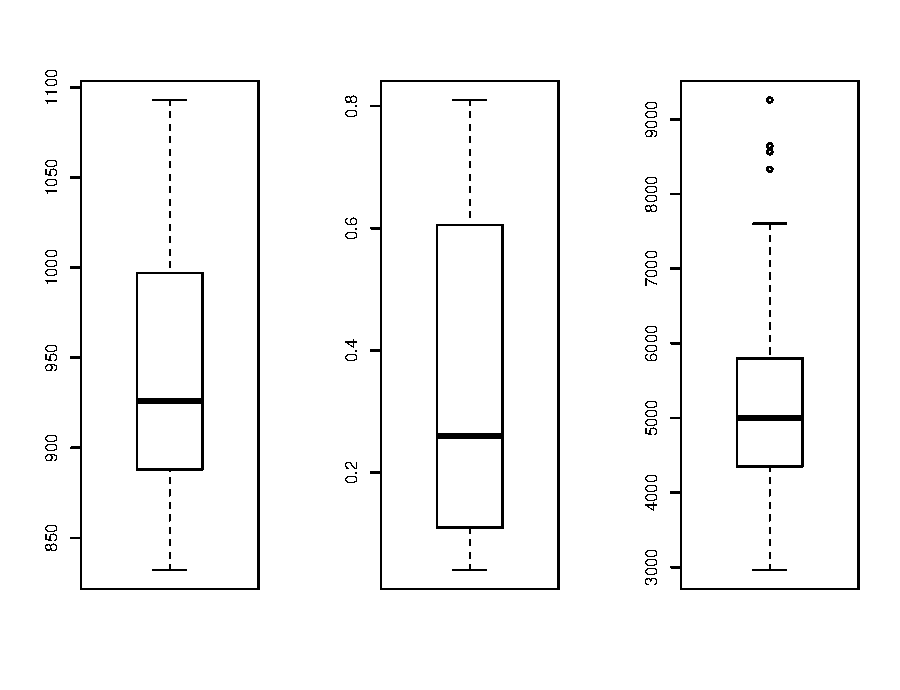
\includegraphics{PaperInR_3-location}
\caption{Location of values}
\label{plot_boxplots}
\end{figure}

As we have a categorical variable, we could create a frequency table:


% Table created by stargazer v.5.2 by Marek Hlavac, Harvard University. E-mail: hlavac at fas.harvard.edu
% Date and time: ����, 1�� 04, 2018 - 9:35:33
\begin{table}[!htbp] \centering 
  \caption{Distribution of Region} 
  \label{table_region} 
\begin{tabular}{@{\extracolsep{5pt}} cc} 
\\[-1.8ex]\hline 
\hline \\[-1.8ex] 
Region & Frequency \\ 
\hline \\[-1.8ex] 
Midwest & $12$ \\ 
N. East & $9$ \\ 
South & $17$ \\ 
West & $13$ \\ 
\hline \\[-1.8ex] 
\end{tabular} 
\end{table} 
It does look better now, right? let's work on testing some hypothesis.



\subsection{Modeling}\label{model}

Here, I propose that the amount of money spent for child per state in the US has an effect on the mean average pupils in a state get in SAT:

\begin{Schunk}
\begin{Sinput}
> reg1=lm(satMean~k12ExpenditurePupil, data = states)
> summary(reg1)
\end{Sinput}
\begin{Soutput}
Call:
lm(formula = satMean ~ k12ExpenditurePupil, data = states)

Residuals:
     Min       1Q   Median       3Q      Max 
-131.811  -38.085    5.607   37.852  136.495 

Coefficients:
                      Estimate Std. Error t value Pr(>|t|)    
(Intercept)          1.061e+03  3.270e+01   32.44  < 2e-16 ***
k12ExpenditurePupil -2.228e-02  6.037e-03   -3.69 0.000563 ***
---
Signif. codes:  0 '***' 0.001 '**' 0.01 '*' 0.05 '.' 0.1 ' ' 1

Residual standard error: 59.81 on 49 degrees of freedom
Multiple R-squared:  0.2174,	Adjusted R-squared:  0.2015 
F-statistic: 13.61 on 1 and 49 DF,  p-value: 0.0005631
\end{Soutput}
\end{Schunk}

Here, I modify the previous model; while I insist that the amount of money spent for child per state in the US has an effect on the mean average pupils in a state get in SAT; I will control the effect the demand per state (as demand were equal accross states). Then,

\begin{Schunk}
\begin{Sinput}
> reg2=lm(satMean~k12ExpenditurePupil+satDemand, data = states)
> summary(reg2)
\end{Sinput}
\begin{Soutput}
Call:
lm(formula = satMean ~ k12ExpenditurePupil + satDemand, data = states)

Residuals:
    Min      1Q  Median      3Q     Max 
-62.921 -24.318   1.741  15.502  75.623 

Coefficients:
                      Estimate Std. Error t value Pr(>|t|)    
(Intercept)          9.898e+02  1.840e+01  53.806  < 2e-16 ***
k12ExpenditurePupil  8.604e-03  4.204e-03   2.046   0.0462 *  
satDemand           -2.538e+02  2.249e+01 -11.283 4.21e-15 ***
---
Signif. codes:  0 '***' 0.001 '**' 0.01 '*' 0.05 '.' 0.1 ' ' 1

Residual standard error: 31.62 on 48 degrees of freedom
Multiple R-squared:  0.7857,	Adjusted R-squared:  0.7768 
F-statistic: 88.01 on 2 and 48 DF,  p-value: < 2.2e-16
\end{Soutput}
\end{Schunk}

Do you like the way my results are shown?...I will improve them later.

Try `uncommenting' the re encoding package \emph{inputenc} on this document header.


\end{document}
